
% This LaTeX was auto-generated from MATLAB code.
% To make changes, update the MATLAB code and republish this document.

\documentclass{article}
\usepackage{graphicx}
\usepackage{color}

\sloppy
\definecolor{lightgray}{gray}{0.5}
\setlength{\parindent}{0pt}

\begin{document}

    
    
\section*{Problem 5.75}

\begin{par}
I used the code from the book
\end{par} \vspace{1em}

\subsection*{Contents}

\begin{itemize}
\setlength{\itemsep}{-1ex}
   \item Setup
   \item A
   \item B
   \item C
   \item D
   \item E
\end{itemize}


\subsection*{Setup}

\begin{verbatim}
clear; close all; clc

[X,Y] = meshgrid(-8:0.1:8);
mux = 0; muy = 0;
\end{verbatim}


\subsection*{A}

\begin{verbatim}
stdx = 3; stdy = 3;
varx = stdx^2; vary=stdy^2;
rho = 0;

X1 = (X-mux)/stdx;
Y1 = (Y-muy)/stdy;

Z = X1.^2-2*rho*X1.*Y1+Y1.^2;
c = 1;

figure(1);
contour(X,Y,Z,c)

title('Std x = Std y');
xlabel('x'); ylabel('y');
axis([-9 9 -9 9]);
\end{verbatim}

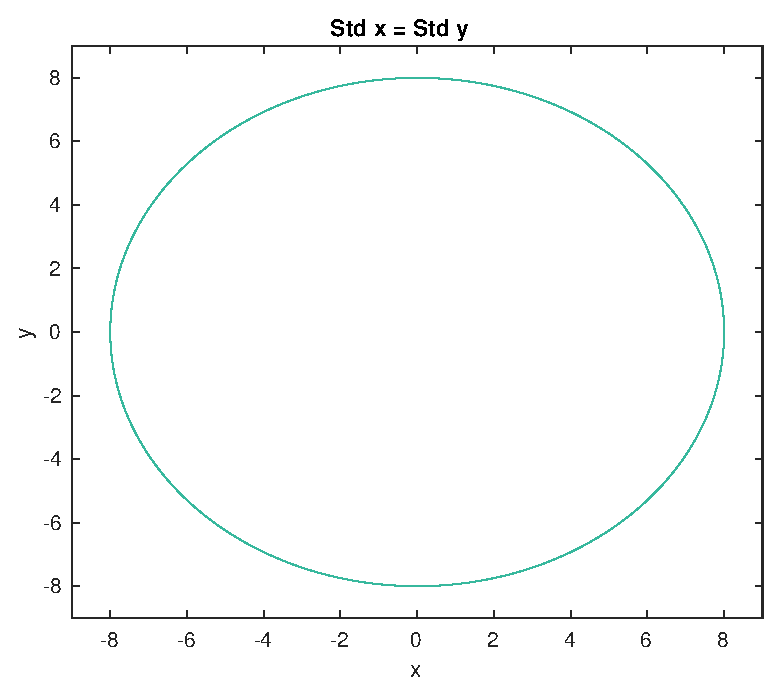
\includegraphics [width=4in]{prob_5_75_01.eps}


\subsection*{B}

\begin{verbatim}
stdx = 1; stdy = 3;
varx = stdx^2; vary=stdy^2;
rho = 0;

X1 = (X-mux)/stdx;
Y1 = (Y-muy)/stdy;

Z = X1.^2-2*rho*X1.*Y1+Y1.^2;
c = 1;

figure(2);
contour(X,Y,Z,c)

title('Std x < Std y');
xlabel('x'); ylabel('y');
\end{verbatim}

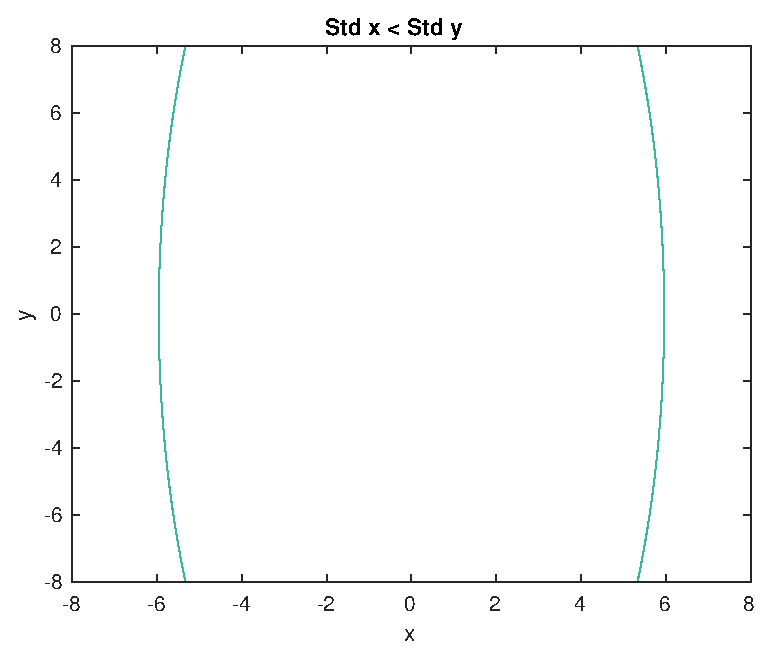
\includegraphics [width=4in]{prob_5_75_02.eps}


\subsection*{C}

\begin{verbatim}
stdx = 3; stdy = 1;
varx = stdx^2; vary=stdy^2;
rho = 0;

X1 = (X-mux)/stdx;
Y1 = (Y-muy)/stdy;

Z = X1.^2-2*rho*X1.*Y1+Y1.^2;
c = 1;

figure(3);
contour(X,Y,Z,c)

title('Std x > Std y');
xlabel('x'); ylabel('y');
\end{verbatim}

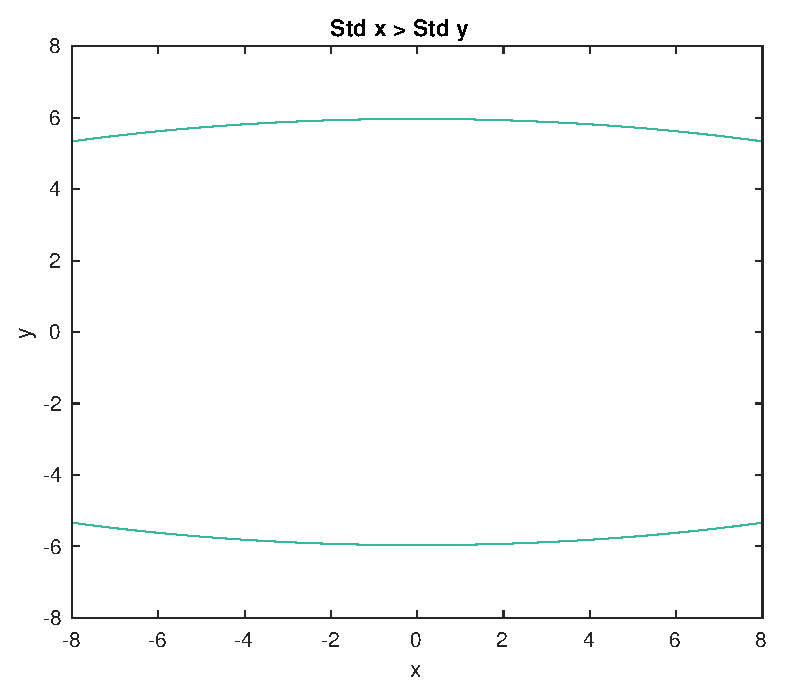
\includegraphics [width=4in]{prob_5_75_03.eps}


\subsection*{D}

\begin{verbatim}
stdx = 3; stdy = 3;
varx = stdx^2; vary=stdy^2;
rho = .5;

X1 = (X-mux)/stdx;
Y1 = (Y-muy)/stdy;

Z = X1.^2-2*rho*X1.*Y1+Y1.^2;
c =1;

figure(4);
contour(X,Y,Z,c)

title('Std x = Std y, Rho != 0');
xlabel('x'); ylabel('y');
\end{verbatim}

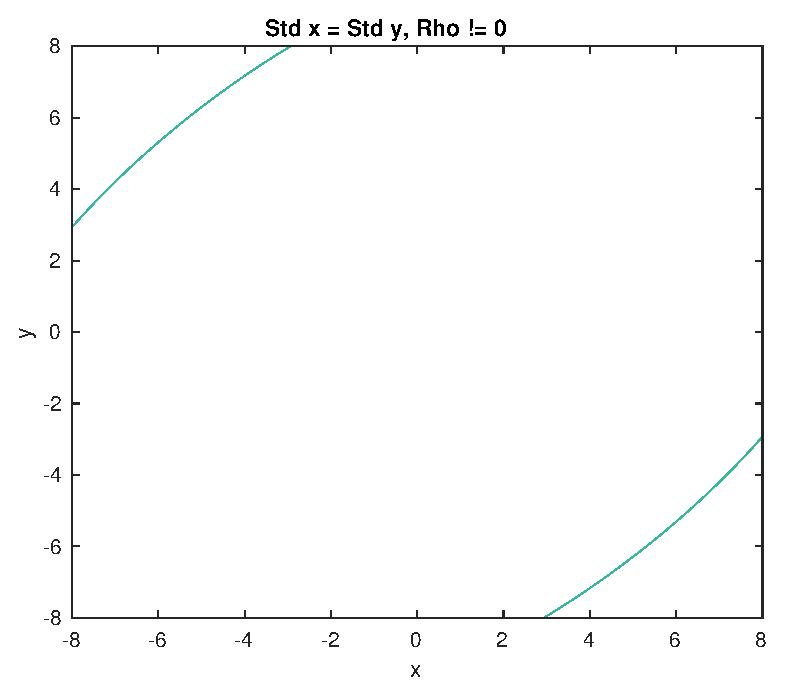
\includegraphics [width=4in]{prob_5_75_04.eps}


\subsection*{E}

\begin{verbatim}
stdx = 3; stdy = 3;
varx = stdx^2; vary=stdy^2;
rho = 0;

X1 = (X-mux)/stdx;
Y1 = (Y-muy)/stdy;

Z = X1.^2-2*rho*X1.*Y1+Y1.^2;
c = [.1 .5 1 2 4 8];

figure(5);
contour(X,Y,Z,c)

title('Std x = Std y, Various C');
xlabel('x'); ylabel('y');
\end{verbatim}

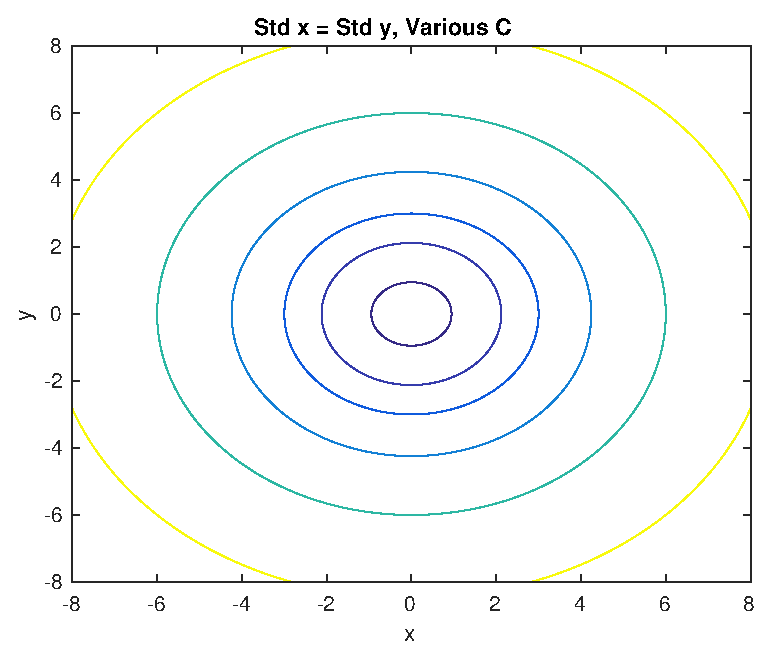
\includegraphics [width=4in]{prob_5_75_05.eps}



\end{document}
    
